\chapter{PROCEDIMENTOS METODOLÓGICOS}

A presente pesquisa aplicada foi desenvolvida através da exploração de casos de
uso tanto da evolução de aplicativos centrais da plataforma GNOME quanto padrões
de design utilizados em outras versões do cliente de torrent Transmission.

Segundo \citeonline{jung2003metodologia}, o objetivo da pesquisa aplicada é
gerar inovação frente a uma demanda ou necessidade, e seu desenvolvimento
consiste na utilização dos conhecimentos adquiridos na pesquisa básica
associados a pesquisa tecnológica, com a finalidade de obter aplicações
práticas.

O produto final desta pesquisa se concretiza na forma de um protótipo funcional
de interface gráfica compatível com os padrões definidos no HIG 3.14 para o
cliente de torrent Transmission.

\section{Estudo longitudinal dos padrões de design nas aplicações}
\label{sec:chronologic-analysis}

Através de pesquisa exploratória com o objetivo de avaliar o processo de
evolução da plataforma GNOME e seu design, foram identificadas aplicações
centrais do GNOME 3.16 que já implementam os padrões de design definidos pelo
HIG \cite{gnome314hig}.

\citeonline{jung2003metodologia} caracteriza a pesquisa exploratória pela
extração de conhecimento sobre um dado fenômeno, sem grande teorização, visando
descobrir práticas e diretrizes alternativas ao conhecimento existente.

Foram escolhidas três aplicações centrais a serem analisadas. Pelo papel
significativo desempenhado na experiência GNOME foram selecionadas as seguintes
aplicações:

\begin{itemize}
    \item Nautilus -- Navegador de Arquivos
    \item Evince -- Visualizador de Documentos Digitais
    \item Gedit -- Editor de Arquivos de Texto
\end{itemize}

Com propósito de avaliar a dinâmica do processo de design do GNOME ao longo do
tempo, um estudo de caráter longitudinal foi elaborado nas três aplicações
escolhidas, através da comparação de duas versões distantes do GNOME e das
aplicações centrais escolhidas.

A montagem do ambiente necessário para a execução do estudo longitudinal foi
facilitada pela distribuição oficial de sistemas operacionais com todo software
necessário para uma experiência GNOME básica, prontos para usar através da
transferência para uma mídia inicializável \cite{gnome2015promo-usb}. Detalhadas
na \autoref{gnome-versions} estão as informações das versões escolhidas, dentre
as disponíveis para estudo.

A soma de verificação de cada arquivo foi utilizada para checar a integridade do
sistema operacional, e todas aplicações foram analisadas na versão oficial --
sem alterações na configuração do sistema, troca de temas, fontes, etc.

\begin{table}[htb]
\ibgetab{
  \caption{Sistemas operacionais e versões do GNOME}
  \label{gnome-versions}
}{
  \begin{tabularx}{\textwidth}{ | l | l | l | X | }
  \hline
  Versão do GNOME & Data de Modificação & Nome do arquivo & Soma de Verificação \\
  \hline
  3.6.0 & 08/10/2012 & GNOME-3.6.0.iso       & MD5:
                                               753c99ce2342f658
                                               65c1f74bc3722e44 \\
  \hline
  3.16  & 25/03/2015 & gnome-3.16.x86-64.iso & SHA256:
                                               4a6185a0aca89f15
                                               8f769d76d5a0086f
                                               0f1e9d709a5d80cd
                                               cf2b0d52d67ab2b2 \\
  \hline
  \end{tabularx}
}{
  \fonte{\cite{gnome2015promo-usb}}
}
\end{table}

Dentre os diversos padrões de design especificados pelo HIG
\cite{hig314patterns} foram selecionados cinco padrões de interesse a serem
analisados no estudo:

\begin{enumerate}
  \item Menu da Aplicação
  \item Janela Primária
  \item Barra de Título
  \item Comutador de Visão
  \item Busca
\end{enumerate}

As variáveis observadas no estudo incluiram, porém não se limitaram a (i) área
útil vs controles, onde foi analisada a razão entre a quantidade de pixels de
área útil versus controles da aplicação e (ii) relocação de funcionalidade,
onde foram analisadas mudanças operacionais em um mais elementos de interface,
sendo estas de caráter quantitativo e qualitativo, respectivamente.

A obtenção da razão área útil versus controles foi feita através da medição em
pixels da janela principal de cada aplicativo Foi considerada área útil a área
do aplicativo na qual a informação principal é apresentada, conforme
exemplificado na \autoref{workarea-chrome-ratio}. No caso do Nautilus, a lista
de arquivos é a área principal, do Evince, o documento apresentado, e no caso do
Gedit, a área de edição de texto.

\begin{figure}[h!]
  \begin{center}
    \caption{\textbf{Medição da razão área útil vs controles}}
    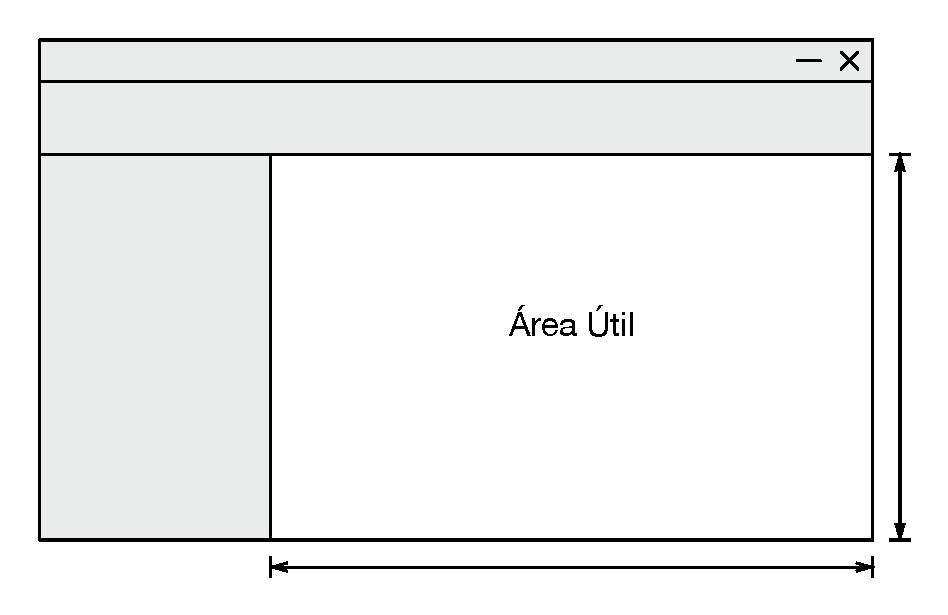
\includegraphics[scale=0.7]{image/workarea-chrome-ratio.eps}
    \fonte{Do Autor}
    \label{workarea-chrome-ratio}
  \end{center}
\end{figure}

A relocação de funcionalidades analisou a transição de um elemento de interface,
onde um menu, por exemplo, pode ter sido transformado em um botão, movido para
outro local, etc.

\section{Proposição de melhorias na interface do Transmission}

\citeonline{de2009client} afirmam que a prototipação de interfaces é uma técnica
de evolução de design que tem como base a constante interação e avaliação dos
resultados. \citeonline[p. 2]{baumer1996user} classifica e separa em quatro
classes os protótipos de interfaces gráficas:

\begin{enumerate}
  \item De apresentação
  \item Funcional
  \item Experimental
  \item Piloto
\end{enumerate}

Pela (i) maleabilidade de implementar estrategicamente ambas interface gráfica e
funcionalidade de um programa, com o propósito de averiguar o funcionamento de
um conceito e (ii) pelo fato do Transmission permitir alterações em seu código-
fonte através de sua licença GPL o protótipo funcional foi escolhido como método
experimental para a geração de propostas de melhorias na interface do
Transmission.

O protótipo funcional foi gerado através de alterações experimentais no código-
fonte do Transmission objetivando modificar sua interface gráfica utilizando
como base as tendências encontradas no estudo logitudinal das aplicações
centrais e também as diretivas estabelecidas no HIG.
